\documentclass[conference]{IEEEtran}
\IEEEoverridecommandlockouts
% The preceding line is only needed to identify funding in the first footnote. If that is unneeded, please comment it out.
\usepackage{cite}
\usepackage{amsmath,amssymb,amsfonts}
\usepackage{algorithmic}
\usepackage{graphicx}
\usepackage{textcomp}
\usepackage{xcolor}
\def\BibTeX{{\rm B\kern-.05em{\sc i\kern-.025em b}\kern-.08em
    T\kern-.1667em\lower.7ex\hbox{E}\kern-.125emX}}
\begin{document}

\title{Nature-Inspired Computing\\Project Report\\}

\author{\IEEEauthorblockN{Ayhem Bouabid}
\IEEEauthorblockA{\textit{DS-01} \\
\textit{Innopolis University}\\
Innopolis, Russian Federation \\
a.bouabid@innopolis.university}
\and
\IEEEauthorblockN{Majid Naser}
\IEEEauthorblockA{\textit{DS-01} \\
\textit{Innopolis University}\\
Innopolis, Russian Federation \\
m.naser@innopolis.university}
\and
\IEEEauthorblockN{Nikolay Pavlenko}
\IEEEauthorblockA{\textit{DS-01} \\
\textit{Innopolis University}\\
Innopolis, Russian Federation \\
n.pavlenko@innopolis.university}
}

\maketitle

\begin{abstract}
tbd
\end{abstract}

\begin{IEEEkeywords}
tbd
\end{IEEEkeywords}

\section{Introduction}
tbd

\section{Related Work}
tbd

\section{Methodology}
tbd

\section{Github link}
tbd

\section{Experiments and Evaluation}
tbd

\section{Analysis and Observations}
tbd

\section{Conclusion}
tbd

\section{References}
tbd

\section{Funni table}

\begin{table}[htbp]
\caption{Table Type Styles}
\begin{center}
\begin{tabular}{|c|c|c|c|}
\hline
\textbf{Table}&\multicolumn{3}{|c|}{\textbf{Table Column Head}} \\
\cline{2-4} 
\textbf{Head} & \textbf{\textit{Table column subhead}}& \textbf{\textit{Subhead}}& \textbf{\textit{Subhead}} \\
\hline
copy& More table copy$^{\mathrm{a}}$& &  \\
\hline
\multicolumn{4}{l}{$^{\mathrm{a}}$Sample of a Table footnote.}
\end{tabular}
\label{tab1}
\end{center}
\end{table}

\section{Funni picture}

\begin{figure}[htbp]
\centerline{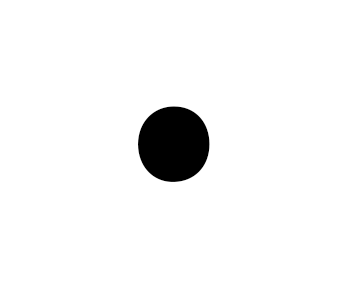
\includegraphics{fig1.png}}
\caption{Example of a figure caption.}
\label{fig}
\end{figure}

\end{document}
